\documentclass[crop,tikz]{standalone}

\usetikzlibrary{automata}

\begin{document}
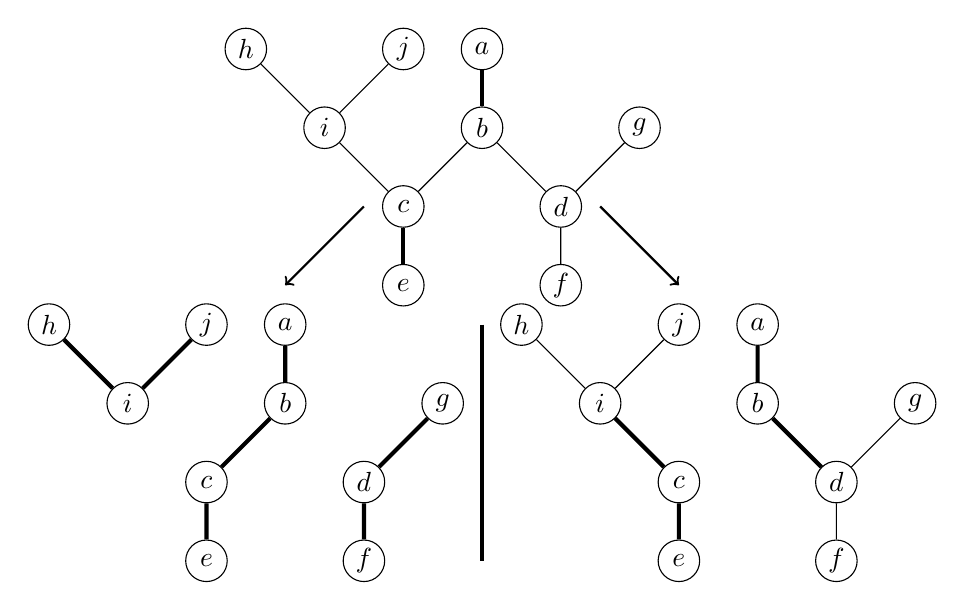
\begin{tikzpicture}
\tikzstyle{vertex}=[draw,shape=circle,inner sep=0pt,minimum size=15pt]
\path (0,0) node[vertex](f0){$a$};
\path (-2,-1) node[vertex](x0){$i$} (-1,-2) node[vertex](x1){$c$} (0,-1) node[vertex](f1){$b$} (1,-2) node[vertex](y1){$d$} (2,-1) node[vertex](y0){$g$};
\path (-1,-3) node[vertex](x2){$e$} (1,-3) node[vertex](y2){$f$};
\path (-3,0) node[vertex](x3){$h$} (-1,0) node[vertex](x4){$j$};
\draw[line width=1.5pt] (f0) -- (f1);
\draw[line width=1.5pt] (x2) -- (x1);
\draw (x0) -- (x1) -- (f1) -- (y1) -- (y2);
\draw (x3) -- (x0) -- (x4);
\draw (y0) -- (y1);

\path (-2.5,-3.5) node[vertex](f0){$a$};
\path (-4.5,-4.5) node[vertex](x0){$i$} (-3.5,-5.5) node[vertex](x1){$c$} (-2.5,-4.5) node[vertex](f1){$b$} (-1.5,-5.5) node[vertex](y1){$d$} (-0.5,-4.5) node[vertex](y0){$g$};
\path (-3.5,-6.5) node[vertex](x2){$e$} (-1.5,-6.5) node[vertex](y2){$f$};
\path (-5.5,-3.5) node[vertex](x3){$h$} (-3.5,-3.5) node[vertex](x4){$j$};
\draw[line width=1.5pt] (f0) -- (f1) -- (x1) -- (x2);
\draw[line width=1.5pt] (x3) -- (x0) -- (x4);
\draw[line width=1.5pt] (y2) -- (y1) -- (y0);

\path (3.5,-3.5) node[vertex](f0){$a$};
\path (1.5,-4.5) node[vertex](x0){$i$} (2.5,-5.5) node[vertex](x1){$c$} (3.5,-4.5) node[vertex](f1){$b$} (4.5,-5.5) node[vertex](y1){$d$} (5.5,-4.5) node[vertex](y0){$g$};
\path (2.5,-6.5) node[vertex](x2){$e$} (4.5,-6.5) node[vertex](y2){$f$};
\path (0.5,-3.5) node[vertex](x3){$h$} (2.5,-3.5) node[vertex](x4){$j$};
\draw[line width=1.5pt] (f0) -- (f1) -- (y1);
\draw[line width=1.5pt] (x0) -- (x1) -- (x2);
\draw (x3) -- (x0) -- (x4);
\draw (y0) -- (y1) -- (y2);

\draw[thick, ->] (-1.5,-2) -- (-2.5,-3);
\draw[thick, ->] (1.5,-2) -- (2.5,-3);

\draw[line width=1.5pt] (0,-3.5) -- (0,-6.5);
\end{tikzpicture}
\end{document}